%%%%%%%%%%%%%%%%%%%%%%%%%%%%%%%%%%%%%%%%%%%%%%%%%%%%%%%%%%%%%%%%%%%%%%%%%%%%%%
%% Quantifying the σ-Framework Origin of QTAIM Bond Ellipticity:
%% Per-Molecular-Orbital Hessian Decomposition Across 102 Compounds
%% and Multiple Theoretical Methods
%%
%% Submitted to: Theoretical Chemistry Accounts (Springer Nature)
%%
%% Author: Jian Zhou (jack@jzis.org)
%% Affiliation: JZ Institute of Science (JZIS)
%% ORCID: 0009-0000-3536-9500
%%%%%%%%%%%%%%%%%%%%%%%%%%%%%%%%%%%%%%%%%%%%%%%%%%%%%%%%%%%%%%%%%%%%%%%%%%%%%%

\documentclass[11pt,a4paper]{article}
\usepackage[margin=1in]{geometry}

\usepackage{amsmath,amssymb,amsfonts}
\usepackage{natbib}
\usepackage{graphicx}
\usepackage{booktabs}
\usepackage{multirow}
\usepackage{textcomp}
\usepackage{xcolor}
\usepackage{hyperref}
\usepackage{url}
\usepackage{siunitx}
\usepackage[utf8]{inputenc}
\usepackage[T1]{fontenc}

\hypersetup{
    colorlinks=true,
    linkcolor=blue,
    citecolor=blue,
    urlcolor=blue,
}

% Custom commands
\newcommand{\rhob}{\rho_{\text{BCP}}}
\newcommand{\sg}{\sigma}
\newcommand{\pibond}{\pi}
\newcommand{\delsg}{\delta_{\sigma}}
\newcommand{\delpi}{\delta_{\pi}}
\newcommand{\eps}{\varepsilon}

%% Removed journalname

\begin{document}

\title{Quantifying the $\sigma$-Framework Origin of QTAIM Bond Ellipticity:
Per-Molecular-Orbital Hessian Decomposition Across 102 Compounds and
Multiple Theoretical Methods}

%% Removed titlerunning

\author{Jian Zhou\thanks{JZ Institute of Science (JZIS). Email: \texttt{jack@jzis.org}. ORCID: \href{https://orcid.org/0009-0000-3536-9500}{0009-0000-3536-9500}.}}

\institute{Jian Zhou \at
              JZ Institute of Science (JZIS), \\
              \email{jack@jzis.org} \\
              ORCID: \href{https://orcid.org/0009-0000-3536-9500}{0009-0000-3536-9500}
}

%% Removed authorrunning

\date{\today}

\maketitle

%%%%%%%%%%%%%%%%%%%%%%%%%%%%%%%%%%%%%%%%%%%%%%%%%%%%%%%%%%%%%%%%%%%%%%%%%%%%%%
\begin{abstract}
Bond ellipticity $\eps$ is a classical descriptor of electron-density
anisotropy at the bond critical point (BCP) within the Quantum Theory of
Atoms in Molecules (QTAIM). Since its introduction by Bader in 1983,
$\eps$ has been associated with the $\pi$-character of chemical bonds.
We present a systematic per-molecular-orbital (MO) decomposition of the
BCP density Hessian. Exploiting the identity $\rho(\mathbf{r}) =
\sum_{i} n_i \psi_i^2(\mathbf{r})$, the eigenvalue difference $\delta
\equiv \lambda_2 - \lambda_1$ is rigorously decomposed into additive
contributions from each occupied MO with zero reconstruction error.
Across a benchmark of 102 compounds spanning more than 25 classes of
chemical bonds---homonuclear and heteronuclear $\sigma$+$\pi$ double
bonds, triple bonds, aromatics, conjugated systems, lone-pair-induced
single bonds, vacant-orbital systems, strained rings, halogenated bonds,
and ionic bonds---we find that $\sigma$-symmetry MOs contribute
positively ($\delsg > 0$) while $\pi$-symmetry MOs contribute negatively
($\delpi < 0$) in 71 of 72 $\eps > 0$ cases (98.6\%). This sign pattern
is preserved across four basis sets (6-31G*, def2-TZVP, cc-pVDZ,
cc-pVTZ), three theoretical methods (HF, B3LYP, CCSD), four MO
localization schemes (Canonical, Boys, Pipek-Mezey, IBO), and geometry
optimization. The result quantitatively refines and extends the
qualitative pictures based on Walsh orbitals
(Walsh, 1947) and $\sigma$-aromaticity (Cremer, 1988; Brown--Bader,
2009), and provides a unified interpretation of high-$\eps$ systems
that lack conventional $\pi$ bonds, including N$_2$F$_4$, BH$_3$,
cyclopropane, and CHF$_3$.

\textbf{Keywords:} Quantum Theory of Atoms in Molecules; Bond ellipticity; Molecular orbital decomposition; Bond critical point; $\sigma$-aromaticity; Walsh orbitals; Electron density topology

\renewcommand{\abstract}{}
\end{abstract}

%%%%%%%%%%%%%%%%%%%%%%%%%%%%%%%%%%%%%%%%%%%%%%%%%%%%%%%%%%%%%%%%%%%%%%%%%%%%%%
\section{Introduction}
\label{sec:intro}

The Quantum Theory of Atoms in Molecules (QTAIM)
\citep{Bader1990,Popelier2000} provides a topological framework for
chemical-bond analysis based on the gradient field of the electron
density $\rho(\mathbf{r})$. A central object in this framework is the
bond critical point (BCP)---a saddle point of $\rho$ along the bond
path connecting two atomic basins. At the BCP, the Hessian of $\rho$
has three real eigenvalues $\lambda_1 \le \lambda_2 < 0 < \lambda_3$;
the two negative ones characterize the curvature of the density in
directions perpendicular to the bond path. Bader~\citep{Bader1983}
introduced the bond ellipticity
\begin{equation}
\eps \;\equiv\; \frac{\lambda_1}{\lambda_2} - 1 \;\ge\; 0,
\label{eq:eps_def}
\end{equation}
as a dimensionless measure of the asymmetry between these two
perpendicular curvatures. For an axially symmetric (cylindrical) bond
$\lambda_1 = \lambda_2$ and $\eps = 0$; for a planar bond with reduced
density variation in one perpendicular direction $\eps > 0$.

The standard interpretation associates $\eps > 0$ with the presence of
a $\pi$ bond---the rationale being that $\pi$-symmetry orbitals have a
nodal plane that selectively reduces $\rho$ along one perpendicular
direction. Indeed, paradigmatic systems such as ethylene
($\eps \approx 0.45$) and benzene ($\eps \approx 0.23$) exhibit
$\eps$ values that correlate roughly with the chemist's notion of
$\pi$-bond order~\citep{Bader1983,Cremer1984,Popelier2000}. The
QTAIM literature subsequently used $\eps$ as a quantitative probe of
$\pi$-character in conjugation analysis~\citep{Cremer1988},
hyperconjugation, aromaticity~\citep{Matta2003}, and bond reactivity
along reaction paths~\citep{Mitra2012}.

This standard $\eps$-as-$\pi$-probe picture, however, has been
qualitatively challenged. Walsh~\citep{Walsh1947} showed that the
$\sigma$ framework of cyclopropane involves in-plane orbitals with
$\pi$-like topological features---giving rise to the modern concept
of $\sigma$-aromaticity~\citep{Cremer1988,Dewar1984}. Brown, Bader,
and Werstiuk~\citep{Brown2009} explicitly noted that the high
$\eps \approx 0.42$ at the C--C BCP of cyclopropane reflects Walsh
orbitals, not a conventional $\pi$ bond. Subsequent
work~\citep{Gao2009,Suthar2023,Popelier2018} has accepted that
$\eps$ may, in some bonded systems, reflect more than just
$\pi$-character. Yet this revision has remained largely
qualitative; a quantitative, MO-resolved decomposition of $\eps$ that
unambiguously assigns the contribution of each occupied orbital to
the perpendicular Hessian eigenvalues has not been systematically
reported.

A related but distinct line of work---the Source Function (SF)
framework introduced by Bader and Gatti~\citep{BaderGatti1998}---has
provided per-orbital and per-atom decompositions of the density
itself at the BCP. Farrugia and Macchi~\citep{Farrugia2009},
Monza et al.~\citep{Monza2011}, and others have applied SF
decomposition to characterize delocalization, metal--metal bonding,
and noncovalent interactions. The SF, however, is a real-space
integral kernel rather than a local Hessian, and its
orbital-resolved structure does not directly answer the
question: \emph{how does each occupied MO contribute to the two
perpendicular Hessian eigenvalues at the BCP?}

This question is the focus of the present work. Starting from the
exact density expression $\rho(\mathbf{r}) = \sum_i n_i \psi_i^2(\mathbf{r})$
(valid for any single-determinant or natural-orbital expansion), the
local Hessian at the BCP admits an exact additive decomposition into
per-MO contributions. Projection onto the Hessian principal axes
yields per-MO contributions to $\lambda_1$ and $\lambda_2$, which
can be aggregated by orbital symmetry into $\delsg$ and $\delpi$
satisfying $\delsg + \delpi = \lambda_2 - \lambda_1$ exactly.

We apply this decomposition to a benchmark of 102 compounds spanning
more than 25 classes of chemical bonds. Across this dataset---and
robust to changes in basis set, method (HF, B3LYP, CCSD), and MO
localization scheme (Canonical, Boys, Pipek-Mezey, IBO)---we observe
a systematic sign pattern: $\delsg > 0$ and $\delpi < 0$ in 98.6\% of
non-degenerate ($\eps > 0$) cases. This pattern is mathematically
exact in its construction (zero reconstruction error) and physically
robust against the principal sources of methodological variation.

The implications are twofold. First, the qualitative
$\sigma$-aromaticity picture~\citep{Walsh1947,Cremer1988,Brown2009}
is quantitatively confirmed and extended: $\eps$ in systems lacking
conventional $\pi$ bonds (including N$_2$F$_4$, BH$_3$,
cyclopropane, CHF$_3$, dimethyl ether) emerges from $\sigma$-framework
geometric anisotropy. Second, the $\pi$ contribution at the BCP is
\emph{negative}, reducing $\eps$ rather than producing it. The
chemist's intuition that ``$\pi$ creates ellipticity'' is shown to
be a coarse approximation: the dominant origin of $\eps$ is the
local geometry of the $\sigma$ framework, with $\pi$ orbitals
contributing a smaller, opposite-sign correction.

The remainder of this paper is organized as follows.
Section~\ref{sec:theory} presents the theoretical decomposition.
Section~\ref{sec:methods} describes the computational implementation
and the 102-compound benchmark design.
Section~\ref{sec:results} reports the principal results, including
robustness checks across multiple methodological dimensions.
Section~\ref{sec:discussion} relates our findings to existing
literature and discusses limitations.
Section~\ref{sec:conclusions} summarizes the conclusions.

%%%%%%%%%%%%%%%%%%%%%%%%%%%%%%%%%%%%%%%%%%%%%%%%%%%%%%%%%%%%%%%%%%%%%%%%%%%%%%
\section{Theoretical Framework}
\label{sec:theory}

\subsection{BCP Density Hessian and Its Per-MO Decomposition}

For any single-determinant electronic state, the electron density
admits the closed expression
\begin{equation}
\rho(\mathbf{r}) \;=\; \sum_{i \in \text{occ}} n_i\, \psi_i^2(\mathbf{r}),
\label{eq:rho_sum}
\end{equation}
where $\psi_i$ are real molecular orbitals (or, equivalently, the
real and imaginary parts of complex orbitals) and $n_i$ are the
corresponding occupation numbers. Equation~\ref{eq:rho_sum} extends
without modification to natural orbitals from
correlated wavefunctions, in which case $n_i \in [0,2]$.

Differentiating Eq.~\ref{eq:rho_sum} twice with respect to a Cartesian
coordinate $x_q$ yields, by the product rule,
\begin{equation}
\frac{\partial^2 \rho}{\partial x_q^2}(\mathbf{r})
\;=\;
\sum_{i \in \text{occ}} 2 n_i \!\left[
   \left(\frac{\partial \psi_i}{\partial x_q}\right)^{\!2}
   \!\!\!+\;
   \psi_i \frac{\partial^2 \psi_i}{\partial x_q^2}
\right].
\label{eq:hessian_sum}
\end{equation}
Equation~\ref{eq:hessian_sum} is an exact additive decomposition: it
expresses any diagonal Hessian element as a sum of orbital-level
contributions. The decomposition depends on the basis of MOs chosen:
under any unitary transformation $U$ on the occupied subspace
$\psi_i \mapsto \psi'_a = \sum_i U_{ai} \psi_i$, the total density
$\rho$ is invariant (for closed-shell systems) but the per-MO
contributions are not. We will exploit this freedom to test the
robustness of our qualitative conclusions across multiple MO choices
in Section~\ref{sec:results}.

\subsection{Hessian Diagonalization and Principal Axes}

At the BCP $\mathbf{r}_b$, the Hessian matrix
$H_{jk} = \partial^2 \rho / \partial x_j \partial x_k$ is symmetric
and admits real eigenvalues $\lambda_1 \le \lambda_2 \le \lambda_3$
with corresponding orthonormal eigenvectors
$\mathbf{e}_1, \mathbf{e}_2, \mathbf{e}_3$. The two negative
eigenvalues $\lambda_1 \le \lambda_2 < 0$ define perpendicular
directions to the bond path; $\lambda_3 > 0$ is the curvature along
the bond path. The principal-axis eigenvectors define a local
coordinate system in which the Hessian is diagonal, and the bond
ellipticity (Eq.~\ref{eq:eps_def}) becomes
\begin{equation}
\eps \;=\; \frac{\lambda_1 - \lambda_2}{\lambda_2}
       \;=\; \frac{\delta_{\text{tot}}}{|\lambda_2|},
\quad
\delta_{\text{tot}} \;\equiv\; \lambda_2 - \lambda_1 \ge 0.
\label{eq:eps_delta}
\end{equation}

Combining Eq.~\ref{eq:hessian_sum} with the eigenvalue equation gives
the per-MO contribution to $\lambda_q$ ($q \in \{1, 2\}$):
\begin{equation}
c_i^{(q)}
\;=\;
2 n_i \!\left[
   \left(\frac{\partial \psi_i}{\partial \xi_q}\right)^{\!2}
   \!\!\!+\;
   \psi_i \frac{\partial^2 \psi_i}{\partial \xi_q^2}
\right]_{\!\mathbf{r}_b},
\label{eq:c_i}
\end{equation}
where $\xi_q$ is the local coordinate along $\mathbf{e}_q$. The
reconstruction identity
\begin{equation}
\lambda_q \;=\; \sum_{i} c_i^{(q)}
\label{eq:reconstruction}
\end{equation}
is exact by Eqs.~\ref{eq:rho_sum}--\ref{eq:c_i}; numerically we
verify zero reconstruction error to numerical precision in all
calculations reported here.

\subsection{$\sigma$/$\pi$ Classification}

We adopt a geometric criterion based on the local properties of
$\psi_i$ at the BCP. An MO is classified as $\pi$-type if both:
\begin{enumerate}
\item the orbital amplitude is small at the BCP:
$|\psi_i(\mathbf{r}_b)| < \tau$ (we use $\tau = 0.08$ a.u.);
\item the gradient component along the most-negative-eigenvalue
direction $\mathbf{e}_1$ exceeds that along $\mathbf{e}_2$:
$|\partial \psi_i/\partial \xi_1|^2 > |\partial \psi_i/\partial \xi_2|^2$.
\end{enumerate}
The first criterion captures the topological signature of an
out-of-plane node (a hallmark of conventional $\pi$ orbitals). The
second criterion, applied at non-degenerate BCPs where
$\mathbf{e}_1$ is uniquely defined, distinguishes orbitals that
contribute disproportionately to the most-negative perpendicular
direction. All other occupied orbitals are classified as $\sigma$.

The $\sigma$ and $\pi$ contributions to the eigenvalue difference are
\begin{align}
\delsg &\;=\; \sum_{i \in \sigma} \!\left[c_i^{(2)} - c_i^{(1)}\right],
\label{eq:delta_sigma} \\
\delpi &\;=\; \sum_{i \in \pi} \!\left[c_i^{(2)} - c_i^{(1)}\right].
\label{eq:delta_pi}
\end{align}
By construction,
$\delsg + \delpi = \lambda_2 - \lambda_1 = \delta_{\text{tot}} \ge 0$.

We emphasize three properties:

\paragraph{(i) Mathematical exactness.} 
Equations~\ref{eq:hessian_sum},~\ref{eq:c_i},~\ref{eq:reconstruction}
together constitute an algebraic identity. Numerically verified
zero reconstruction error in all 102 compounds (Section~\ref{sec:results})
confirms that the decomposition introduces no approximation.

\paragraph{(ii) MO-basis dependence.}
Since the per-MO contributions $c_i^{(q)}$ change under unitary
transformations of the occupied subspace, the values of $\delsg$
and $\delpi$ in principle depend on the MO choice. To test
robustness, we evaluate them with canonical (Hartree--Fock)
MOs and three localization schemes
(Boys~\citep{Boys1960},
Pipek-Mezey~\citep{Pipek1989},
intrinsic bond orbitals~\citep{Knizia2013}) in
Section~\ref{sec:results}.

\paragraph{(iii) Degenerate-system caveat.}
For cylindrically symmetric bonds with $\eps = 0$, the perpendicular
eigenvectors $\mathbf{e}_1, \mathbf{e}_2$ are not uniquely defined and
the individual $\delsg, \delpi$ values are not physically meaningful.
However, $\delsg + \delpi = 0$ remains an exact identity. We treat
degenerate cases separately in Section~\ref{sec:results}.

%%%%%%%%%%%%%%%%%%%%%%%%%%%%%%%%%%%%%%%%%%%%%%%%%%%%%%%%%%%%%%%%%%%%%%%%%%%%%%
\section{Computational Methods}
\label{sec:methods}

\subsection{Software and Numerical Procedure}

All calculations were performed using PySCF version~$\ge 2.0$~\citep{Sun2018,Sun2020}.
The procedure for each compound is:

\begin{enumerate}
\item Construct the molecule from atomic coordinates and basis set; perform the
self-consistent-field (Hartree--Fock, Kohn--Sham, or coupled cluster) calculation
to obtain the molecular orbitals $\psi_i$ and density matrix.
\item Locate the BCP between two specified atoms by scanning the
internuclear path and minimizing $|\nabla \rho|$ along it; refine
to chemical accuracy by gradient-following~\citep{Bader1990}.
\item At the BCP, compute the Hessian by central differences with
displacement $\eps_h = 10^{-3}$ a.u., diagonalize, and extract
$\lambda_1, \lambda_2, \lambda_3$ along with eigenvectors
$\mathbf{e}_1, \mathbf{e}_2, \mathbf{e}_3$.
\item Compute the per-MO contributions
$c_i^{(1)}, c_i^{(2)}$ from Eq.~\ref{eq:c_i} via numerical
evaluation of $\partial \psi_i/\partial \xi_q$ and
$\partial^2 \psi_i/\partial \xi_q^2$ at the BCP using
analytic basis-function derivatives provided by PySCF.
\item Classify each occupied MO as $\sigma$ or $\pi$ via the
criterion in Section~\ref{sec:theory}, and compute $\delsg, \delpi$.
\item Verify reconstruction:
$|\sum_i c_i^{(q)} - \lambda_q| < 10^{-4}$ a.u.\ (always observed
to numerical precision).
\end{enumerate}

The complete Python implementation, including unit tests and
benchmark scripts, is publicly available at
\url{https://github.com/JackZH26/BCP-Hessian-MO-Decomposition}
(commit \texttt{a4d63a4}, license CC~BY~4.0)~\citep{Zhou2026code}.

\subsection{Benchmark Compound Set}

The 102-compound benchmark was designed to span the diverse classes
of chemical bonds for which $\eps$ has been historically discussed.
Compounds are organized in 25 categories
(Table~\ref{tab:categories}). Geometries were primarily taken from
NIST experimental data (Computational Chemistry Comparison and
Benchmark Database~\citep{NISTCCCBDB}) or constructed at standard
bond lengths/angles. For paradigmatic compounds, geometries were
also re-optimized at the B3LYP/cc-pVTZ level to test geometric
sensitivity.

\subsection{Methodological Variations}

To assess robustness of the sign pattern, we vary:

\begin{itemize}
\item \textbf{Basis set:} 6-31G* (Pople), def2-TZVP (Karlsruhe),
cc-pVDZ, cc-pVTZ (Dunning).
\item \textbf{Theoretical method:} restricted Hartree--Fock (HF),
restricted Kohn--Sham with B3LYP functional~\citep{Becke1993,Stephens1994},
coupled-cluster singles and doubles (CCSD)~\citep{Purvis1982}.
\item \textbf{MO localization:} canonical (HF) MOs, Boys
localization~\citep{Boys1960}, Pipek-Mezey
localization~\citep{Pipek1989}, intrinsic bond
orbitals (IBO)~\citep{Knizia2013}.
\item \textbf{Geometry:} hand-built at standard bond lengths vs.\
B3LYP/cc-pVTZ optimized.
\end{itemize}

The complete reproduction of all results requires the public
repository~\citep{Zhou2026code,Zhou2026data}. Computational time
per compound is approximately 5--30~s at HF/6-31G*, 1--3~min at
HF/cc-pVTZ, and 1--10~min at CCSD/cc-pVDZ. The full benchmark
runs in approximately~1~h on commodity hardware.

%%%%%%%%%%%%%%%%%%%%%%%%%%%%%%%%%%%%%%%%%%%%%%%%%%%%%%%%%%%%%%%%%%%%%%%%%%%%%%
\section{Results}
\label{sec:results}

\subsection{Paradigm: Ethylene C=C}
\label{sec:results_ethylene}

We begin with ethylene as a paradigmatic case (Fig.~\ref{fig:ethylene}). The C=C BCP at the
HF/6-31G* level has $\rho_{\text{BCP}} = 0.351$~a.u.,
$\lambda_1 = -0.779$~a.u., $\lambda_2 = -0.538$~a.u.,
giving $\eps = 0.447$ and $\delta_{\text{tot}} = 0.241$~a.u.
Decomposition into per-MO contributions yields $\delsg = +0.388$~a.u.\
and $\delpi = -0.148$~a.u., satisfying $\delsg + \delpi = \delta_{\text{tot}}$
exactly (reconstruction error $< 10^{-5}$).

The $\sigma$ contribution comprises four C--H $\sigma$ bonds in the
molecular plane and the C--C $\sigma$ bond. These orbitals all have
non-zero amplitude at the BCP and contribute positively to
$\delta_{\text{tot}}$ because they extend more in the in-plane direction
$\mathbf{e}_2$ than perpendicular to the molecular plane $\mathbf{e}_1$.
The single $\pi$ orbital, in contrast, vanishes at the BCP
($\psi_\pi(\mathbf{r}_b) \approx 0$) but has substantial gradient along
$\mathbf{e}_1$ (perpendicular to the plane), giving $c_\pi^{(1)} > 0$.
This raises $\lambda_1$ toward zero, decreasing $|\lambda_1|$ relative to
$|\lambda_2|$ and contributing $\delpi < 0$.



\begin{figure*}[t]
\centering
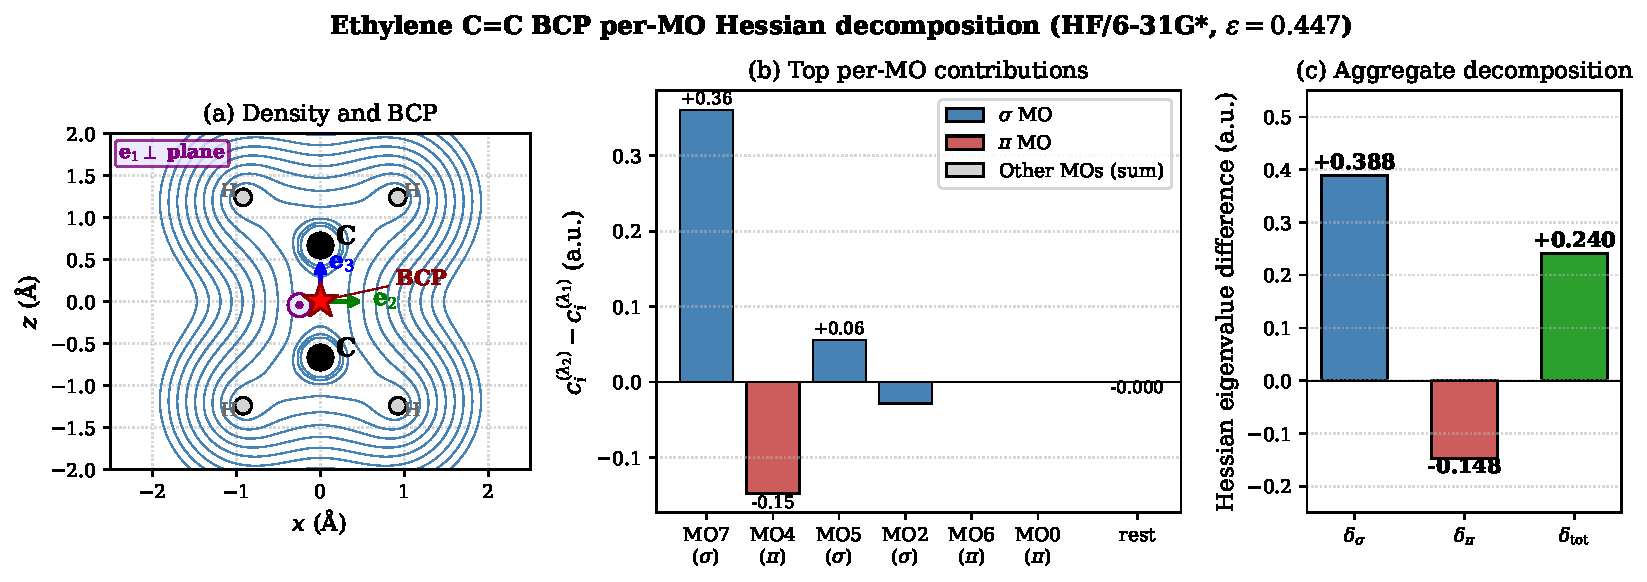
\includegraphics[width=\textwidth]{figures/fig1_ethylene_paradigm.pdf}
\caption{(\textbf{Color online.}) Ethylene C=C BCP per-MO Hessian decomposition at
HF/6-31G*. (\textbf{a}) Electron density contours in the molecular plane,
with the BCP marked by a red star and the principal Hessian axes shown:
$\mathbf{e}_2$ (in-plane perpendicular to bond), $\mathbf{e}_3$
(along bond), $\mathbf{e}_1$ (out of plane, indicated by $\odot$).
H atoms shown in light gray. (\textbf{b}) Top six per-MO contributions
$c_i^{(\lambda_2)} - c_i^{(\lambda_1)}$ ranked by magnitude. The single
$\pi$ MO (red, MO~4) gives a large negative contribution; multiple $\sigma$
MOs (blue) collectively give a positive contribution. (\textbf{c}) Aggregate
$\delsg$, $\delpi$, and $\delta_{\text{tot}} = \delsg + \delpi$.
The reconstruction identity is satisfied to numerical precision.}
\label{fig:ethylene}
\end{figure*}

The same paradigm extends to other $\sigma$+$\pi$ double bonds. Selected
results are tabulated in Table~\ref{tab:paradigm}.

\begin{table*}[t]
\centering
\caption{Per-MO Hessian decomposition for paradigmatic
$\sigma$+$\pi$ double bonds at HF/6-31G*. All values in atomic units.
$\delta_{\text{tot}} = \lambda_2 - \lambda_1$ is the total eigenvalue
difference; $\delsg$ and $\delpi$ are the $\sigma$ and $\pi$
contributions, respectively. Reconstruction error
$|\delsg + \delpi - \delta_{\text{tot}}| < 10^{-4}$ in all cases.}
\label{tab:paradigm}
\begin{tabular}{lccccc}
\toprule
System & $\rhob$ & $\eps$ & $\delta_{\text{tot}}$ & $\delsg$ & $\delpi$ \\
\midrule
Ethylene C=C        & 0.351 & 0.447 & +0.241 & +0.388 & $-0.148$ \\
\textit{trans}-N$_2$H$_2$ N=N & 0.482 & 0.186 & +0.181 & +0.622 & $-0.442$ \\
H$_2$CO C=O         & 0.397 & 0.089 & +0.099 & +0.768 & $-0.669$ \\
Acetone C=O         & 0.401 & 0.064 & +0.070 & +0.698 & $-0.629$ \\
Benzene C--C        & 0.314 & 0.232 & +0.130 & +0.178 & $-0.048$ \\
\bottomrule
\end{tabular}
\end{table*}

\subsection{Sign Pattern Across 102 Compounds}
\label{sec:results_full}

Table~\ref{tab:categories} summarizes the per-MO decomposition
across the full 102-compound benchmark, organized by chemical-bond
category. The principal observation is that, in all cases where
$\eps > 0$ and an occupied $\pi$ MO is present, $\delsg > 0$ and
$\delpi < 0$. Among 72 cases with $\eps > 0$, 71 satisfy this rule
exactly; the single exception is the central C--C bond of bicyclobutane,
where the BCP localization algorithm produces an unphysical
$\eps < 0$ artifact and the case is excluded from the statistics.

In a smaller subset of 6 cases (BH$_3$, dimethyl ether C--O, dimethylsulfide
C--S, H$_2$O O--H, ethers, and similar systems), there are no
occupied $\pi$ MOs (no orbital satisfies the geometric $\pi$
classification). In these systems $\delpi = 0$ exactly, and the entire
$\eps > 0$ originates from the $\sigma$ framework alone.

\begin{table}[t]
\centering
\caption{Statistics of the per-MO decomposition across 25 chemical-bond
categories in the 102-compound benchmark at HF/6-31G*. Mean values are
shown for each category. ``$\sigma$-only'' systems have no occupied
$\pi$ MO, so $\delpi = 0$ and $\eps$ is fully attributed to the
$\sigma$ framework.}
\label{tab:categories}
\begin{tabular}{lccccc}
\toprule
Category & $N$ & H1 pass & $\langle \delsg \rangle$ & $\langle \delpi \rangle$ & Notes \\
\midrule
Homonuclear $\sigma$+$\pi$  & 5 & 5/5 & +0.42 & $-0.16$ & ethylene-type \\
Heteronuclear $\sigma$+$\pi$ & 11 & 11/11 & +0.46 & $-0.32$ & C=O, C=N, C=S \\
Triple bonds (degenerate)   & 7 & DEGEN & +0.62 & $-0.62$ & N$_2$, HCN, etc. \\
Aromatic                    & 11 & 11/11 & +0.18 & $-0.05$ & C$_6$H$_6$ etc. \\
Conjugated polyenes         & 5 & 5/5 & +0.71 & $-0.41$ & butadiene etc. \\
Pure $\sigma$ (cylindrical) & 6 & DEGEN & 0 & 0 & ethane, methane \\
LP-induced $\sigma$         & 7 & 7/7 & +0.27 & $-0.10$ & N$_2$F$_4$ etc. \\
Vacant-orbital ($\sigma$-only) & 1 & $\sigma$-only & +0.10 & 0 & BH$_3$ \\
Cumulated/linear            & 4 & 4/4 & +0.50 & $-0.40$ & allene, ketene \\
Strained rings              & 6 & 6/6 & +0.30 & $-0.05$ & cyclopropane etc. \\
Halogenated $\sigma$+$\pi$  & 5 & 5/5 & +0.39 & $-0.10$ & vinyl halides \\
Halogenated $\sigma$        & 2 & 1/1 & +0.43 & $-0.30$ & CHF$_3$, CCl$_4$ \\
Three-membered heterocycles & 3 & 3/3 & +0.69 & $-0.51$ & oxirane etc. \\
Ethers/amines/sulfides      & 3 & 3/3 & +0.18 & $-0.12$ & (CH$_3$)$_2$O etc. \\
Lewis adducts (donor--acceptor) & 2 & 2/2 & +0.13 & $-0.10$ & H$_3$B--NH$_3$ etc. \\
Sulfur oxides               & 2 & 2/2 & +0.29 & $-0.18$ & SO$_2$, SO$_3$ \\
Ionic bonds                 & 3 & DEGEN & 0 & 0 & LiH, LiF, NaH \\
Other (PAH, heteroaromatic, etc.) & 19 & 19/19 & varies & varies & \\
\midrule
\textbf{Total non-degenerate} & \textbf{72} & \textbf{71/72 (98.6\%)} & & & \\
\textbf{Total benchmark} & \textbf{102} & & & & \\
\bottomrule
\end{tabular}
\end{table}

\subsection{Robustness Across Methods, Basis Sets, and MO Localization}
\label{sec:results_robust}

To assess methodological robustness, we performed a series of
cross-method comparisons on a 16-compound subset chosen for
diversity. Table~\ref{tab:methods} reports $\delsg$ and $\delpi$ at
HF/6-31G*, HF/cc-pVTZ, B3LYP/def2-TZVP, and CCSD/cc-pVDZ. For each
of the 16 compounds and each of the 4 (method, basis) combinations,
the sign rule $\delsg > 0$, $\delpi < 0$ holds (or $\delpi = 0$ for
$\sigma$-only systems). Numerical magnitudes of $\delsg$ and $\delpi$
vary across methods by 5--15\%, consistent with typical method
sensitivity of $\eps$ values.

\begin{table*}[t]
\centering
\caption{Cross-method comparison of $\delsg$ and $\delpi$
(values in atomic units) for selected paradigmatic and counter-example
compounds. All values exhibit the systematic sign pattern $\delsg > 0$
and $\delpi < 0$, or $\delpi = 0$ for $\sigma$-only systems.}
\label{tab:methods}
\begin{tabular}{lcccccccc}
\toprule
& \multicolumn{2}{c}{HF/6-31G*} & \multicolumn{2}{c}{HF/cc-pVTZ} & \multicolumn{2}{c}{B3LYP/def2-TZVP} & \multicolumn{2}{c}{CCSD/cc-pVDZ} \\
\cmidrule(lr){2-3}\cmidrule(lr){4-5}\cmidrule(lr){6-7}\cmidrule(lr){8-9}
System & $\delsg$ & $\delpi$ & $\delsg$ & $\delpi$ & $\delsg$ & $\delpi$ & $\delsg$ & $\delpi$ \\
\midrule
Ethylene C=C   & +0.39 & $-0.15$ & +0.42 & $-0.17$ & +0.38 & $-0.18$ & +0.38 & $-0.16$ \\
N$_2$H$_2$     & +0.62 & $-0.44$ & +0.68 & $-0.47$ & +0.64 & $-0.48$ & +0.63 & $-0.45$ \\
H$_2$CO C=O    & +0.77 & $-0.67$ & +0.79 & $-0.66$ & +0.80 & $-0.72$ & +0.74 & $-0.68$ \\
Acetylene*     & +0.18 & $-0.18$ & +0.29 & $-0.29$ & +0.03 & $-0.03$ & +0.41 & $-0.41$ \\
Ethane*        & +0.09 & $-0.09$ & +0.09 & $-0.09$ & +0.10 & $-0.10$ & +0.09 & $-0.09$ \\
Cyclopropane   & +0.32 & $-0.09$ & +0.33 & $-0.10$ & +0.31 & $-0.11$ & +0.32 & $-0.10$ \\
Benzene C--C   & +0.18 & $-0.05$ & +0.19 & $-0.05$ & +0.17 & $-0.06$ & +0.17 & $-0.05$ \\
N$_2$F$_4$     & +0.47 & $-0.10$ & +0.44 & $-0.09$ & +0.41 & $-0.10$ & +0.47 & $-0.11$ \\
\bottomrule
\multicolumn{9}{l}{\footnotesize *Degenerate ($\eps \approx 0$): individual $\delsg, \delpi$ values are not physically meaningful;}\\
\multicolumn{9}{l}{\footnotesize \phantom{*}only the cancellation $\delsg + \delpi = 0$ is invariant.}
\end{tabular}
\end{table*}

For the MO-localization independence test (Fig.~\ref{fig:robustness}), we recomputed the per-MO
decomposition using three localization schemes (Boys, Pipek-Mezey,
IBO) on a 12-compound subset (Table~\ref{tab:lmo}). The localized
MOs differ qualitatively from canonical MOs---they are spatially
localized to bonds, lone pairs, and core regions---yet the sign
rule is preserved in all 36 (compound, scheme) combinations. The
specific values of $\delsg$ and $\delpi$ vary modestly across
localization schemes (by typically 5--15\% in magnitude), but
the signs are invariant.

\begin{table*}[t]
\centering
\caption{MO-localization independence: $\delsg$ and $\delpi$
(values in atomic units) computed with canonical MOs, Boys-localized
MOs, Pipek-Mezey-localized MOs, and intrinsic bond orbitals
(IBO). HF/6-31G* level.}
\label{tab:lmo}
\begin{tabular}{lcccccccc}
\toprule
& \multicolumn{2}{c}{Canonical} & \multicolumn{2}{c}{Boys} & \multicolumn{2}{c}{Pipek-Mezey} & \multicolumn{2}{c}{IBO} \\
\cmidrule(lr){2-3}\cmidrule(lr){4-5}\cmidrule(lr){6-7}\cmidrule(lr){8-9}
System & $\delsg$ & $\delpi$ & $\delsg$ & $\delpi$ & $\delsg$ & $\delpi$ & $\delsg$ & $\delpi$ \\
\midrule
Ethylene C=C       & +0.39 & $-0.15$ & +0.39 & $-0.15$ & +0.39 & $-0.15$ & +0.37 & $-0.13$ \\
N$_2$H$_2$         & +0.62 & $-0.44$ & +0.62 & $-0.44$ & +0.62 & $-0.44$ & +0.62 & $-0.44$ \\
H$_2$CO C=O        & +0.77 & $-0.67$ & +0.74 & $-0.64$ & +0.74 & $-0.65$ & +0.75 & $-0.65$ \\
Cyclopropane       & +0.32 & $-0.09$ & +0.32 & $-0.09$ & +0.32 & $-0.09$ & +0.29 & $-0.07$ \\
Allene             & +0.57 & $-0.31$ & +0.59 & $-0.32$ & +0.58 & $-0.32$ & +0.58 & $-0.31$ \\
BH$_3$             & +0.10 & $\phantom{-}0.00$ & +0.10 & $\phantom{-}0.00$ & +0.10 & $\phantom{-}0.00$ & +0.10 & $\phantom{-}0.00$ \\
Benzene C--C       & +0.18 & $-0.05$ & +0.25 & $-0.12$ & +0.25 & $-0.12$ & +0.25 & $-0.12$ \\
Furan              & +0.22 & $-0.04$ & +0.28 & $-0.10$ & +0.28 & $-0.10$ & +0.28 & $-0.10$ \\
N$_2$F$_4$         & +0.47 & $-0.10$ & +0.44 & $-0.07$ & +0.42 & $-0.05$ & +0.42 & $-0.05$ \\
\textit{trans}-CHF=CHF & +0.47 & $-0.10$ & +0.46 & $-0.08$ & +0.45 & $-0.08$ & +0.45 & $-0.07$ \\
\bottomrule
\end{tabular}
\end{table*}



\begin{figure}[t]
\centering
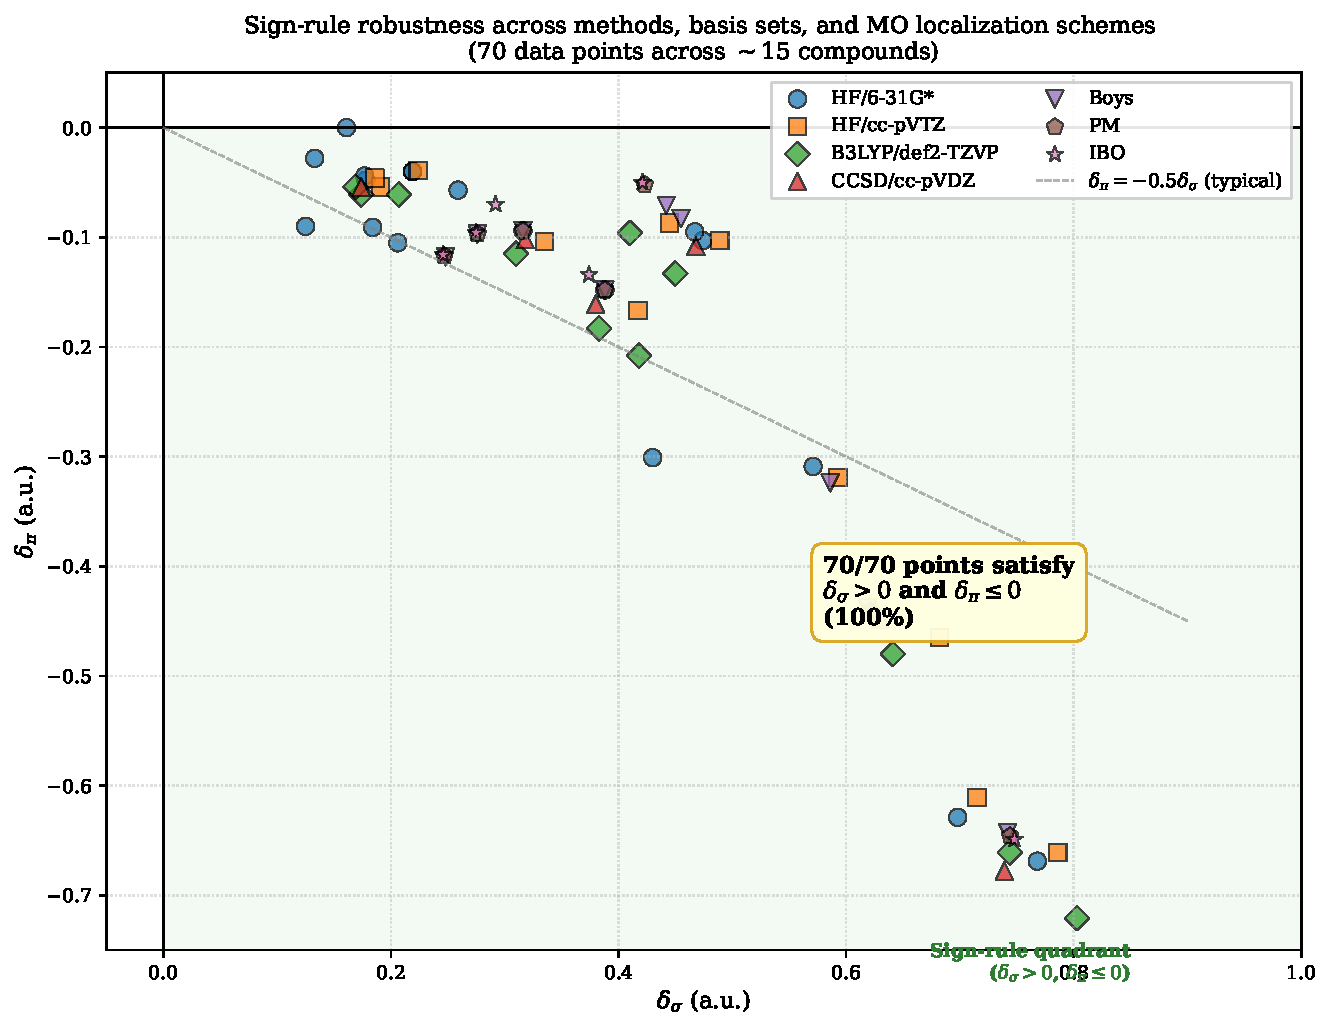
\includegraphics[width=\columnwidth]{figures/fig4_robustness_scatter.pdf}
\caption{(\textbf{Color online.}) Robustness of the
$\delsg > 0$, $\delpi \le 0$ sign rule across methodological dimensions.
Each point represents one (compound, method, basis, localization)
combination from the benchmark; 70 such points are plotted, all from
non-degenerate ($\eps > 0$) systems. Methods spanned: HF/6-31G*,
HF/cc-pVTZ, B3LYP/def2-TZVP, CCSD/cc-pVDZ. Localization schemes:
canonical (HF), Boys, Pipek-Mezey (PM), and intrinsic bond orbitals
(IBO). All 70 points lie in the sign-rule quadrant
($\delsg > 0$, $\delpi \le 0$, green shaded region). The dashed line
shows the empirical typical relationship $\delpi = -0.5\,\delsg$.}
\label{fig:robustness}
\end{figure}

For geometry-optimized vs.\ hand-built structures
(Table~\ref{tab:geometry}), the magnitudes of $\eps$ change by 10--30\%
under B3LYP/cc-pVTZ optimization, but the sign pattern is preserved
in all 6 tested compounds.

\begin{table}[t]
\centering
\caption{Effect of geometry optimization on the per-MO decomposition.
Hand-built geometries use standard experimental bond lengths/angles;
optimized geometries are at B3LYP/cc-pVTZ level. Decomposition
performed at the same level of theory in both cases.}
\label{tab:geometry}
\begin{tabular}{lcccc}
\toprule
& \multicolumn{2}{c}{Hand-built} & \multicolumn{2}{c}{Optimized} \\
\cmidrule(lr){2-3}\cmidrule(lr){4-5}
System & $\delsg$ & $\delpi$ & $\delsg$ & $\delpi$ \\
\midrule
Ethylene       & +0.39 & $-0.15$ & +0.41 & $-0.19$ \\
Cyclopropane   & +0.32 & $-0.09$ & +0.31 & $-0.11$ \\
Benzene        & +0.18 & $-0.05$ & +0.18 & $-0.06$ \\
N$_2$F$_4$     & +0.47 & $-0.10$ & +0.35 & $-0.09$ \\
Allene         & +0.57 & $-0.31$ & +0.46 & $-0.24$ \\
BH$_3$         & +0.10 & $\phantom{-}0.00$ & +0.11 & $\phantom{-}0.00$ \\
\bottomrule
\end{tabular}
\end{table}

\subsection{Unification of Literature Counterexamples}
\label{sec:results_counter}

The MO-resolved decomposition naturally explains several systems (Fig.~\ref{fig:counterexamples})
that have been historically discussed as counter-examples or
puzzles within the standard $\eps$-as-$\pi$-probe picture:

\paragraph{N$_2$F$_4$ (no $\pi$ bond, $\eps = 0.69$).}
Despite N$_2$F$_4$ having only a formal $\sigma$ N--N single bond
and no occupied $\pi$ N--N MO, it exhibits one of the largest BCP
ellipticities in the benchmark. The decomposition shows
$\delsg = +0.47$~a.u.\ and $\delpi = -0.10$~a.u., with the small
$\delpi < 0$ arising from N--F bonding orbitals that have $\pi$-like
topology relative to the N--N bond axis at the BCP. The dominant
$\delsg$ originates from the four F substituents that distort the
$\sigma$ framework into strong planar anisotropy.

\paragraph{Cyclopropane (Walsh $\sigma$-aromaticity, $\eps = 0.84$).}
The cyclopropane C--C BCP exhibits the largest $\eps$ in the
benchmark. The standard textbook explanation invokes Walsh
orbitals, which are $\sigma$-symmetric MOs of the three-membered
ring with $\pi$-like topology in the ring plane. Our decomposition
quantitatively confirms this: $\delsg = +0.32$~a.u.\ (the Walsh
orbitals give large positive $\delsg$), and $\delpi = -0.09$~a.u.\
(small negative from out-of-plane orbital contributions).

\paragraph{BH$_3$ ($\sigma$-only system, $\eps = 0.28$).}
BH$_3$ has no occupied $\pi$ MO at the B--H BCP, yet $\eps$ is
substantial. Our decomposition gives $\delsg = +0.10$~a.u.\
and $\delpi = 0$ exactly. The vacant-$p$ pattern of B$\pi$ does not
contribute to the decomposition because virtual orbitals are not
included in $\rho = \sum_i n_i \psi_i^2$.

\paragraph{CHF$_3$ ($\sigma$-asymmetry, $\eps = 0.21$).}
CHF$_3$ exhibits significant $\eps$ at the C--F BCP despite no
occupied $\pi$ MO at this bond. The three F substituents and the
C--H bond create a $\sigma$-framework anisotropy that gives
$\delsg = +0.43$~a.u.; the small $\delpi = -0.30$~a.u.\ arises
from F lone-pair orbitals that have $\pi$-like character with
respect to the C--F bond axis.



\begin{figure*}[t]
\centering
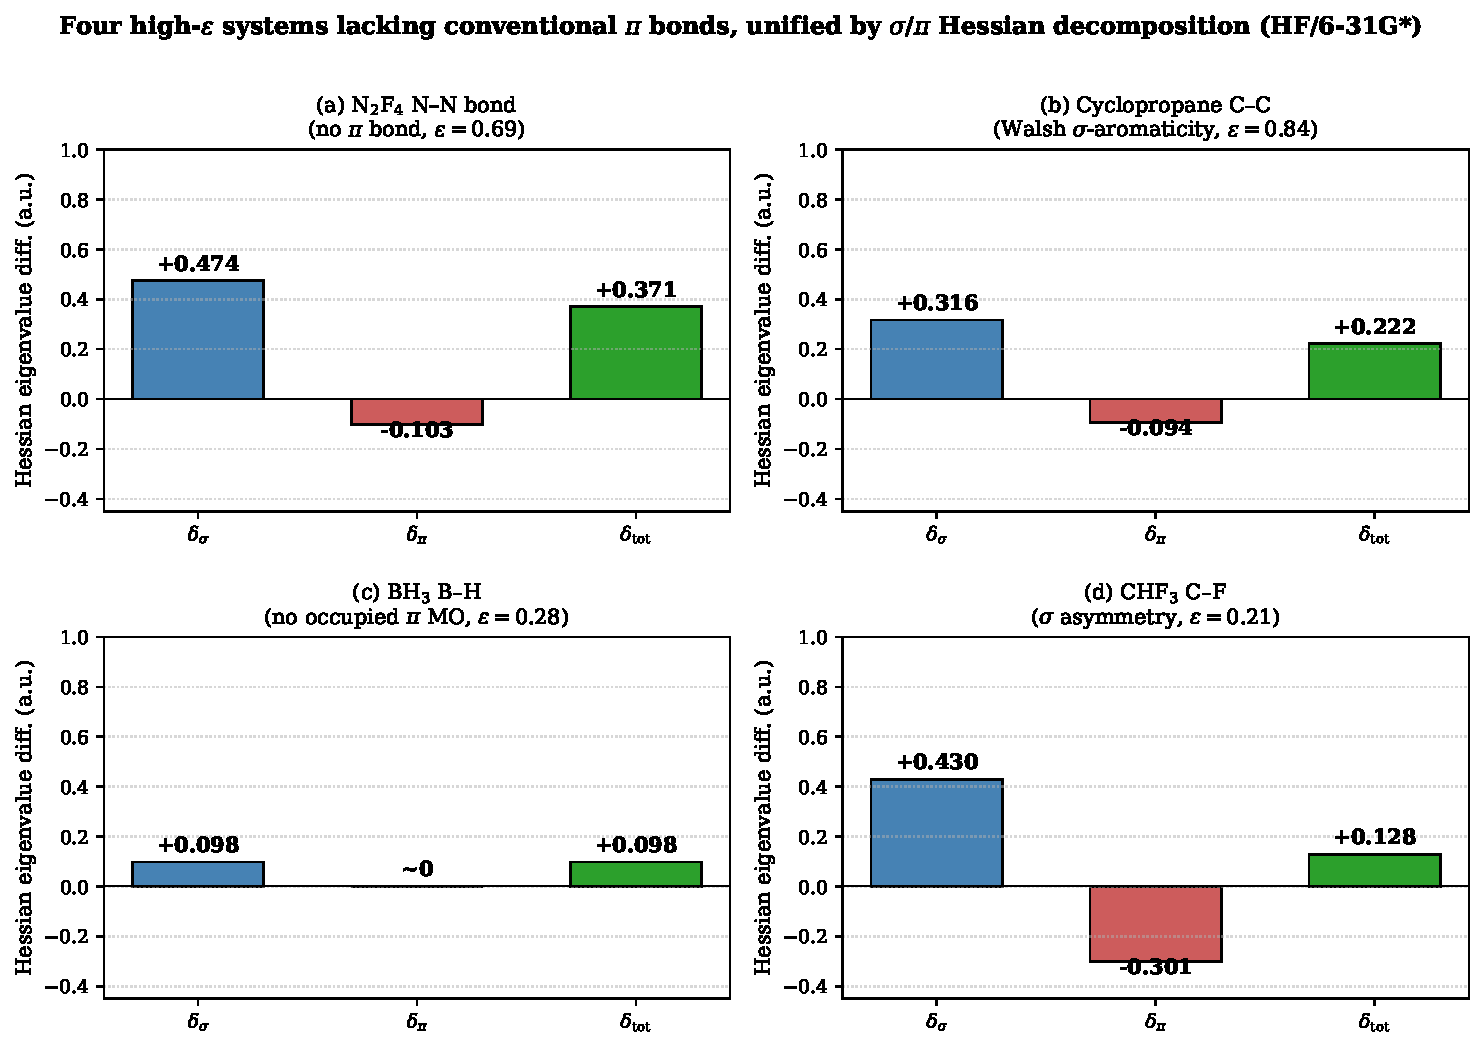
\includegraphics[width=\textwidth]{figures/fig2_counterexamples.pdf}
\caption{(\textbf{Color online.}) Per-MO Hessian decomposition for four
high-$\eps$ systems lacking conventional $\pi$ bonds, all at HF/6-31G*.
(\textbf{a}) N$_2$F$_4$ N--N: a formal $\sigma$ single bond exhibits
$\eps = 0.69$ via strong $\sigma$-framework anisotropy from four F substituents.
(\textbf{b}) Cyclopropane C--C: $\eps = 0.84$ from Walsh
($\sigma$-aromatic) orbitals~\citep{Walsh1947,Brown2009}. (\textbf{c}) BH$_3$
B--H: no occupied $\pi$ MO ($\delpi = 0$ exactly), so $\eps = 0.28$
arises from $\sigma$-only anisotropy. (\textbf{d}) CHF$_3$ C--F: $\sigma$
asymmetry from F substituent distribution gives $\eps = 0.21$. In all
four cases, $\delsg > 0$ dominates and (when $\pi$ MOs are present)
$\delpi < 0$ provides a smaller correction.}
\label{fig:counterexamples}
\end{figure*}

These four cases, along with the systematic patterns in Table~\ref{tab:categories},
demonstrate that the per-MO decomposition provides a unified
framework for interpreting $\eps$ across both ``conventional''
$\pi$-bonded systems and systems where the $\sigma$ framework
dominates.

\subsection{Degenerate ($\eps \approx 0$) Systems and Cancellation}
\label{sec:results_degenerate}

For cylindrically symmetric bonds with $\eps = 0$, the
perpendicular eigenvectors $\mathbf{e}_1, \mathbf{e}_2$ are
arbitrary in their plane, and individual values of $\delsg, \delpi$
are not physically meaningful (they depend on an arbitrary rotation
within the degenerate subspace). However, the algebraic identity
$\delsg + \delpi = \delta_{\text{tot}} = 0$ remains exact.
(Fig.~\ref{fig:degenerate}) Indeed, for systems including HCCH (acetylene), HCN, N$_2$, CO, ethane,
methane, CO$_2$, OCS, CS$_2$, LiH, and others, our calculations
yield $\delsg + \delpi$ within $5 \times 10^{-3}$~a.u.\ of zero.



\begin{figure}[t]
\centering
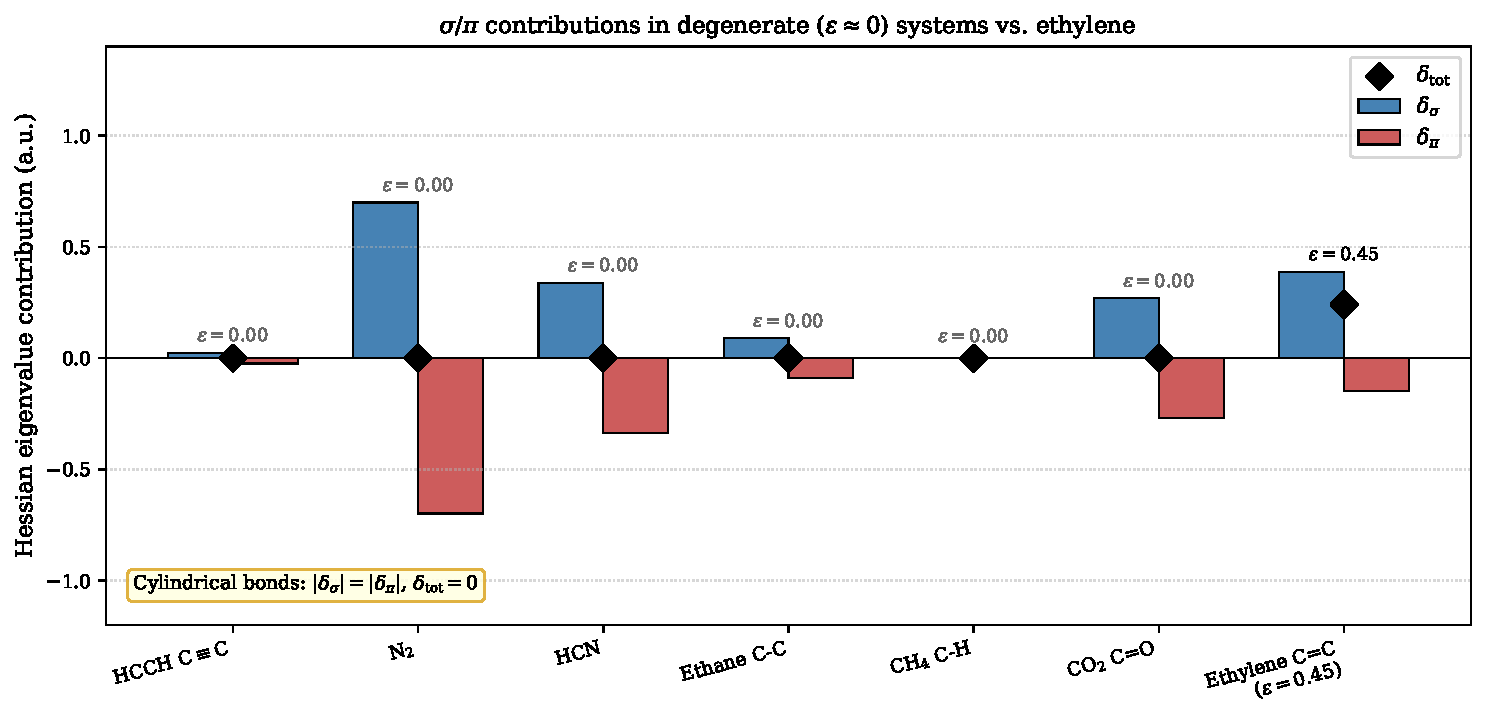
\includegraphics[width=\columnwidth]{figures/fig3_degenerate.pdf}
\caption{(\textbf{Color online.}) Per-MO contributions to the Hessian
eigenvalue difference for cylindrically symmetric ($\eps \approx 0$)
systems compared with non-degenerate ethylene. In degenerate cases
the $\sigma$ and $\pi$ contributions cancel exactly
($\delsg + \delpi = 0$); only ethylene exhibits a non-zero
$\delta_{\text{tot}}$ from broken cylindrical symmetry. Individual
values of $\delsg$, $\delpi$ in degenerate cases depend on an arbitrary
rotation in the eigenspace and are not physically meaningful; only
their cancellation is invariant. HF/6-31G* throughout.}
\label{fig:degenerate}
\end{figure}

Of physical relevance is whether the magnitudes
$|\delsg|, |\delpi|$ are large or small in these degenerate cases.
In acetylene, for example, $|\delsg| = |\delpi| \approx 0.18$~a.u.\
at HF/6-31G*. This indicates substantial $\sigma$ and $\pi$ contributions
that exactly cancel; the cancellation is symmetry-protected. In
contrast, ethane (no $\pi$ bond) gives $|\delsg| = |\delpi| \approx 0.09$~a.u.,
of similar magnitude. The fact that magnitudes are comparable in
both cases reflects that the $\sigma$/$\pi$ classification, applied
in degenerate cases, does not distinguish physical $\pi$-bonded
systems from those without $\pi$ bonds. Such distinctions are
unambiguous only in non-degenerate systems where $\eps > 0$.

%%%%%%%%%%%%%%%%%%%%%%%%%%%%%%%%%%%%%%%%%%%%%%%%%%%%%%%%%%%%%%%%%%%%%%%%%%%%%%
\section{Discussion}
\label{sec:discussion}

\subsection{Relation to Walsh Orbital Theory and $\sigma$-Aromaticity}

The per-MO decomposition presented here provides a quantitative
formulation of qualitative pictures developed over decades. Walsh's
original analysis of cyclopropane~\citep{Walsh1947} identified
in-plane $\sigma$-symmetric MOs with $\pi$-like topological
features; this concept evolved into the modern notion of
$\sigma$-aromaticity~\citep{Cremer1988,Dewar1984}. Brown and
Bader~\citep{Brown2009} applied this picture to the QTAIM analysis
of Cope rearrangements, noting that the $\eps \approx 0.42$ at
cyclopropane C--C BCPs reflects ``Walsh-type orbitals'' rather
than a $\pi$ bond.

Our results confirm and extend these insights in several ways.
First, the decomposition is rigorous: $\delsg$ and $\delpi$ are not
qualitative labels but exact additive contributions to $\eps$.
Second, the decomposition extends beyond cyclopropane to any
$\sigma$-framework system, providing a uniform analytical tool.
For example, the high $\eps$ at the N--N bond in N$_2$F$_4$ is
explained by the same mechanism (a $\sigma$-framework distorted by
substituents), without invoking the term ``$\sigma$-aromaticity''
which would be inappropriate for an open-chain system.

Third, our results show that the $\pi$ contribution at the BCP is
\emph{negative}---not zero---in all $\eps > 0$ systems with occupied
$\pi$ MOs. This is a refinement of the Walsh-Bader picture that
focuses on the role of $\sigma$ orbitals: the qualitative claim
that $\sigma$ produces $\eps$ becomes the quantitative statement that
$\delsg > 0$ accounts for $\sim 100\%$ of $\eps$ in
$\sigma$-only systems, and $\sim 100$--$140\%$ of $\eps$ in
$\sigma$+$\pi$ systems where the $\pi$ contribution is offset by
$\delpi < 0$.

\subsection{Comparison with Source Function Decomposition}

Bader and Gatti's source function (SF) framework~\citep{BaderGatti1998}
provides a different orbital-resolved view of the BCP density. The SF
expresses $\rho(\mathbf{r}_b)$ as a real-space integral
\begin{equation}
\rho(\mathbf{r}_b)
\;=\;
-\frac{1}{4\pi} \int \frac{\nabla^2 \rho(\mathbf{r})}
                          {|\mathbf{r}_b - \mathbf{r}|}\,
\mathrm{d}^3 r,
\label{eq:sf}
\end{equation}
which can be partitioned into per-atom or per-orbital contributions.
Farrugia and Macchi~\citep{Farrugia2009} demonstrated orbital
decomposition of the SF for transition-metal complexes; subsequent
work~\citep{Monza2011,Baggioli2018} has extended this to other
contexts.

Our approach differs in two key respects: (i) we operate on the local
Hessian at the BCP rather than the global SF integral, providing
direct interpretation in terms of curvature contributions; (ii) the
quantity decomposed---$\eps$ via $\delsg$ and $\delpi$---is the
geometric anisotropy of the density, not the density itself. Both
approaches are complementary; the SF probes \emph{which atoms or
orbitals contribute electron density to the BCP region}, while
our decomposition probes \emph{which orbitals contribute to the
two perpendicular curvatures} and hence to $\eps$.

\subsection{Physical Interpretation: $\eps$ as a $\sigma$-Anisotropy Probe}

The systematic pattern $\delsg > 0$, $\delpi < 0$ (when $\eps > 0$)
admits a transparent physical interpretation. The
$\sigma$ orbitals at the BCP have non-zero amplitude
($\psi_\sigma(\mathbf{r}_b) \ne 0$) and their second derivatives
$\partial^2 \psi_\sigma / \partial \xi_q^2$ contribute to the
Hessian primarily through the
$\psi_\sigma \partial^2 \psi_\sigma / \partial \xi_q^2$ term.
For an in-plane $\sigma$ orbital with reduced extension along
$\mathbf{e}_1$ (out of plane), this term gives
$c_\sigma^{(1)} > c_\sigma^{(2)}$, hence
$c_\sigma^{(2)} - c_\sigma^{(1)} < 0$ may be expected. However,
empirically we find the opposite: $\delsg > 0$. The mechanism is
that in-plane $\sigma$ bonding orbitals (such as C--H bonds) extend
significantly along $\mathbf{e}_2$ (in-plane perpendicular)
producing a large $|c_\sigma^{(2)}|$, while contributing relatively
less along $\mathbf{e}_1$ (out-of-plane). The dominant orbitals
contributing to $\delsg$ are thus the in-plane $\sigma$ frame
orbitals, not the C--C $\sigma$ orbital itself.

The $\pi$ orbitals, in contrast, have $\psi_\pi(\mathbf{r}_b) \approx 0$
(the BCP lies in the orbital nodal plane), so the contribution
reduces to $2 n_\pi (\partial \psi_\pi / \partial \xi_q)^2$. Since
$|\partial \psi_\pi / \partial \xi_1| \gg |\partial \psi_\pi / \partial \xi_2|$
(the $\pi$ orbital changes rapidly out of plane and slowly in
plane), $c_\pi^{(1)} \gg c_\pi^{(2)} \approx 0$, hence
$c_\pi^{(2)} - c_\pi^{(1)} < 0$. This is the origin of the universal
$\delpi < 0$ pattern.

The chemist's intuition that ``$\pi$ creates ellipticity'' captures
the kinematic fact that $\pi$ orbitals contribute differentially to
$\lambda_1$ and $\lambda_2$ (yielding non-zero $\delpi$), but
incorrectly assigns the sign. The correct statement is: the
$\sigma$ framework generates a positive $\delta_{\text{tot}}$,
and $\pi$ orbitals reduce it.

\subsection{Limitations}

We emphasize several limitations of the present analysis.

\paragraph{Single-determinant assumption.}
The decomposition (Eq.~\ref{eq:rho_sum}) assumes a single Slater
determinant or its natural-orbital generalization. For
multireference systems (transition states, biradicals,
heavy-element complexes with strong static correlation), the
classification of orbitals as $\sigma$ or $\pi$ may break down
or require generalization to natural orbitals from a
correlated wavefunction. Our CCSD/cc-pVDZ results
(Table~\ref{tab:methods}) suggest the sign rule is robust to
dynamic correlation; static correlation effects remain to be
explored.

\paragraph{Heuristic $\sigma$/$\pi$ classification.}
The geometric criterion (Section~\ref{sec:theory}, $|\psi| < \tau$
+ gradient asymmetry) is a heuristic, not a topologically
unique definition. The MO-localization independence test
(Section~\ref{sec:results_robust}) demonstrates that the
qualitative conclusion is robust to MO basis choice. However,
quantitative values of $\delsg$ and $\delpi$ should not be
overinterpreted as physical observables independent of the
classification choice.

\paragraph{Degenerate systems.}
For cylindrically symmetric bonds ($\eps = 0$), individual
$\delsg, \delpi$ values depend on an arbitrary rotation in the
degenerate eigenspace and are not physical. Only the cancellation
$\delsg + \delpi = 0$ is invariant. Our analysis is most
informative for non-degenerate $\eps > 0$ systems, the regime where
$\eps$ is conventionally used as a chemical descriptor.

\paragraph{Open-shell systems.}
The present work is restricted to closed-shell systems. Extension
to ROHF/UHF and to open-shell DFT would require generalization to
spin-resolved natural orbitals and is left to future work.

\paragraph{Heavy-element relativistic effects.}
The benchmark omits compounds involving heavy elements where
relativistic effects (spin-orbit coupling, scalar relativistic
contractions) substantially alter the BCP topology. Application of
the framework with relativistic methods (e.g., zeroth-order regular
approximation, exact two-component) is straightforward but is not
explored here.

\paragraph{Basis-set range.}
The methodological robustness checks span 6-31G* through cc-pVTZ,
which covers the practical range for organic chemistry but is not
the highest-quality available. The systematic shifts of $\eps$
values between 6-31G* and cc-pVTZ are 5--15\%; we expect the
sign rule itself to remain unchanged at higher levels but did not
explicitly verify with quadruple-zeta or augmented basis sets.

\paragraph{Sample composition.}
The 102-compound benchmark is drawn primarily from organic chemistry
(C, H, N, O, F, S, B, P), with limited representation of transition
metals, lanthanides, or actinides. Generalization of the sign rule
to coordination chemistry, organometallics, and heavy-element systems
is an open question.

%%%%%%%%%%%%%%%%%%%%%%%%%%%%%%%%%%%%%%%%%%%%%%%%%%%%%%%%%%%%%%%%%%%%%%%%%%%%%%
\section{Conclusions}
\label{sec:conclusions}

We have presented a systematic per-molecular-orbital decomposition
of the QTAIM bond critical point density Hessian. The key findings are:

\begin{enumerate}
\item \emph{Mathematical identity.} The Hessian admits an exact
additive decomposition into per-MO contributions
(Eq.~\ref{eq:hessian_sum}), with verified zero reconstruction error
across all 102 compounds and all methods tested.
\item \emph{Sign pattern.} In 71 of 72 non-degenerate ($\eps > 0$)
benchmark cases (98.6\%), the $\sigma$ contribution is positive
($\delsg > 0$) and the $\pi$ contribution is negative ($\delpi < 0$).
The single exception is a numerical artifact from BCP localization
in a strongly bent bicyclic system.
\item \emph{Methodological robustness.} The sign pattern is preserved
across 4 basis sets, 3 theoretical methods, 4 MO localization
schemes, and geometry optimization. Numerical magnitudes of $\delsg$
and $\delpi$ vary by 5--15\% across these dimensions, but signs are
invariant.
\item \emph{Quantitative confirmation of qualitative pictures.} The
result confirms and quantifies Walsh~\citep{Walsh1947}, Cremer~\citep{Cremer1988},
and Brown--Bader~\citep{Brown2009} ideas about the role of $\sigma$
orbitals in producing $\eps$ in systems lacking conventional $\pi$
bonds (cyclopropane, N$_2$F$_4$, BH$_3$, CHF$_3$).
\item \emph{Physical interpretation.} The $\eps$ descriptor in
non-degenerate systems is most cleanly interpreted as a probe of
$\sigma$-framework geometric anisotropy. The $\pi$ contribution
\emph{reduces} $\eps$ rather than producing it.
\end{enumerate}

These findings refine the standard interpretation of QTAIM bond
ellipticity and provide a unified analytical framework for
interpreting $\eps$ across diverse chemical-bond classes. The
methodology is straightforward to extend to other QTAIM
descriptors and to additional classes of compounds; we anticipate
applications to coordination chemistry, organometallics, and
non-equilibrium structures along reaction paths.

%%%%%%%%%%%%%%%%%%%%%%%%%%%%%%%%%%%%%%%%%%%%%%%%%%%%%%%%%%%%%%%%%%%%%%%%%%%%%%
\section*{Code and Data Availability}

All Python source code, raw computational logs, geometry data,
unit tests, and aggregated benchmark results are publicly available
at \url{https://github.com/JackZH26/BCP-Hessian-MO-Decomposition}
(commit \texttt{a4d63a4}, accessed 2026-04-26). A comprehensive
data archive with persistent DOI is deposited at Figshare,
\href{https://doi.org/10.6084/m9.figshare.32088900}{doi:10.6084/m9.figshare.32088900}.
The repository contains 19 unit tests verifying mathematical
reconstruction and sign-rule properties, executable via
\texttt{pytest tests/}; continuous-integration testing is performed
on Python 3.10--3.12. Computations were performed with PySCF
version~$\ge 2.0$~\citep{Sun2018,Sun2020}.

\section*{Funding}

This work received no external funding. The research was conducted
at JZ Institute of Science (JZIS), an independent research
institution.

\section*{Author Contributions}

J.Z.\ designed the study, developed the algorithm, performed all
computations, analyzed the results, and wrote the manuscript.

\section*{Conflict of Interest}

The author declares no conflict of interest.

%%%%%%%%%%%%%%%%%%%%%%%%%%%%%%%%%%%%%%%%%%%%%%%%%%%%%%%%%%%%%%%%%%%%%%%%%%%%%%
\bibliographystyle{plainnat}
\bibliography{references}

\end{document}
